% !TeX root = ../main.tex
% -*- coding: utf-8 -*-

\chapter{绪论}
\label{1}


\section{研究背景与意义}

近年来,科技迅速发展,计算能力得到显著提升,我们正在进入人工智能(Artificial Intelligence, AI)\cite{winston1984artificial}的时代。随着互联网的的快速发展,产生了海量的数据,得益于深度神经网络(Deep neural network, DNN)\cite{sze2017efficient}强大的数据处理能力,DNN已经成为应用最广泛的人工智能方法之一。自DNN在计算机视觉\cite{he2016identity,cortes2015advances,simonyan2014very},语音识别\cite{nassif2019speech},自然语言处理\cite{collobert2011natural,wu2016google,xiong2016achieving}等方面上突破性应用以来,使用DNN的应用数量呈爆炸式增长。这些DNN应用被应用到从自动驾驶\cite{chen2015deepdriving}到癌症检测\cite{esteva2017dermatologist}到玩复杂的游戏\cite{silver2017mastering}等无数应用中。并且在许多这些领域中,DNN现在已经能够超越人类的准确性。

DNN在许多领域取得巨大成功,为人类社会生活带来极大便利的同时,也带来了非常严重的侵犯知识产权问题。训练一个大型的高性能的DNN模型都离不开该领域专家的专业知识、规模巨大的数据集以及大量的训练时间和强大的计算资源,具体体现在以下三个方面:
\begin{enumerate}
	\renewcommand{\labelenumi}{\theenumi)}
	\item 人力资源,对于不同场景不同目的的DNN模型,需要不同领域的知识,包含对模型结构的设计分析、模型参数的调试校验等;
	\item 大量的训练数据,模型所有者要在特定领域训练出一个高性能的模型,通常需要该领域大量的数据,并且需要覆盖到应用场景中的各种情况,这些数据的获取和整理本身就需要昂贵的价格,有的领域的数据还涉及到隐私性问题;
	\item 昂贵的计算资源和大量的训练时间,DNN模型的规模越来越大,层数越来越多,需要的训练时间也越多,并且训练过程中也需要越来越多的计算资源支持,才能对网络权重等进行精确的调整,这些都是巨额的经济成本。如GPT-3\cite{brown2020language},包含了1750亿参数,仅训练成本需花费460万美元以上。
\end{enumerate}
所以高性能DNN模型是模型所有者智慧的结晶,同时需要高额的经济开销,模型所有者享有DNN模型的知识产权。

模型所有者出于学术目的将DNN模型放到开源社区上。或者,使用机器学习即服务(Machine Learning as a Service, MLaaS)的商业模式,即MLaaS平台通过训练好的DNN模型来向用户提供应用程序接口(Application Programming Interface, API),用户可以通过支付一定的费用来使用API。或者,训练好的DNN模型将成为像我们日常商品一样的消费品,它们由不同的公司或个人进行训练,由不同的供应商分发,最终由用户消费。这样的方式极大的方便了科研工作者和一般的消费者,但是不法分子却可以以比模型所有者低很多的成本复制一个替代模型,用于自己盈利。
\begin{figure}[htbp]%%图,[htbp]是浮动格式
	\centering
	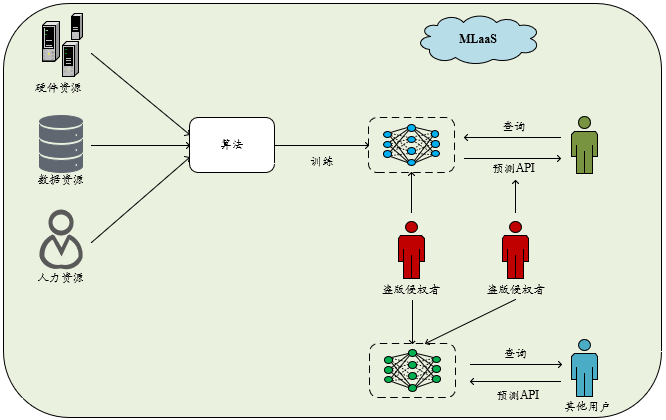
\includegraphics[width=15cm,height=9cm]{DNN模型服务和盗窃.png}
	%	\centerline{原始样本}
	\setlength{\abovecaptionskip}{5mm} %图片标题与图片距离
	\caption{DNN模型服务和盗窃}
	\label{DNN模型服务和盗窃}
	\end {figure}

\section{相关研究现状}

研究问题

研究现状

\section{本文主要工作}

揭示\cite{maini2021dataset}现有问题,确认数据驱动推断所有权的有效性

利用对抗性样本抵御模型窃取

基于DCGAN生成私有数据

广泛实验验证有效性

\section{本文组织架构}

第一章

第二章

第三章

第四章

第五章

第六章